% Partie 1.3 - 6LoWPAN %

\subsection{6LoWPAN}

Cette partie à pour but de présenter le protocole 6LoWPAN ainsi que la norme 802.15.4 utilisée dans les couches basses de 6LoWPAN. Nous avons utilisé pour cette étude un article publié par TI \cite{demystified}.

\subsubsection{802.15.4}

Ce standard de l'\textbf{IEEE} est définie sur deux couches du \textbf{modèle OSI} : la couche physique et la couche MAC. Il est à la base de différents protocoles IoT (notamment ZigBee) qui implémentent des couches supérieures différentes. 

Le framework de base prévoie un rayon de communication de dix mètres pour un débit allant jusqu'à 250 kbit/s. Il est bien sûr possible de réduire la puissance d'émission (le rayon) et de diminuer le débit pour réduire la consommation électrique. L'idée derrière cette réduction drastique est de quand même de conserver une bonne fiabilité.

Comme Wi-Fi (802.11), 802.15.4 utilise comme méthode d’accès \textbf{CSMA/CA} au niveau 2 pour éviter les collisions et intègre plusieurs mécanisme pour la sécurisation des communications. Certains appareils peuvent aussi intégrer des modules d'optimisation de la consommation, de détection de la qualité de la liaison ainsi que la puissance de réception. 

Les appareils conformes à la norme 802.15.4 peuvent désormais utiliser trois bandes de fréquences : 868, 915 et 2~450 MHz. Cela permet de se conformer plus facilement aux normes en vigueur dans chaque pays qui ont des lois en la matière différente. Il n'y a pas de législation mondiale a ce propos.

Le standard défini deux types de nœud :

\begin{description}
	\item[les \textit{Full-Function Devices} (FFD)] peuvent aussi bien servir de coordinateur dans le PAN que comme nœud simple. Ils sont doté d'un module de communication qui permet de retransmettre des trames (faire du routage) ;
	\item[les \textit{Reduced-Function Devices} (RFD)] sont prévues pour être extrêmement simples et possèdent peu de ressources. À cause de cela, il ne peuvent que communiquer avec les FFD et ne peuvent pas être les coordinateurs.
\end{description}

Dans le réseau chaque équipement se voit attribuer un identifiant de 16 bits unique qui permet de faire du routage de niveau 2.

\subsubsection{6LoWPAN}

6LoWPAN est l'acronyme d'\textit{IPv6 over Low power Wireless Personal Area Networks}, ce veut dire Ipv6 au dessus de réseau personnelle sans-fil basse consommation. l'idée principale derrière ce protocole était d'amener IP à tous types d'appareils. 

Aussi, 6LoWPAN n'est spécifié qu'avec IPv6, ce qui fait que l'utilisation d'IPv4 dans un réseau utilisant 6LoWPAN est impossible. Grâce à cela les \textit{edge routers} peuvent utiliser des mécanisme de transition pour connecter des réseaux 6LoWPAN et IPv4 comme \textbf{NAT64}.

Sur un réseau 6LoWPAN le \textit{border/edge router} réalise 3 actions :
\begin{enumerate}
	\item l'échange de données entre les appareils du réseau local et l'Internet (un autre réseau IP) ;
	\item l'échange de données en local ;
	\item la génération et la maintient du réseau.
\end{enumerate}

Ensuite l'un des énormes avantages de 6LoWPAN, du fait de l'utilisation d'IP, est le routage de niveau 3 (couche réseau). Avec 6LoWPAN il n'y pas besoin de maintenir une connexion au niveau applicatif, au contraire de ZigBee, Z-Wave ou Bluetooth qui requiert des passerelles applicatives pour accéder à Internet. En d'autre terme, l'équivalent du \textit{edge router} doit comprendre les protocoles utilisés au niveau applicatif. Cela réduit fortement la charge de travail du routeur.

La \cref{comparison} donne une comparaison des différentes piles utilisées par les protocoles cités précédemment.

\begin{figure}[H]
\centering
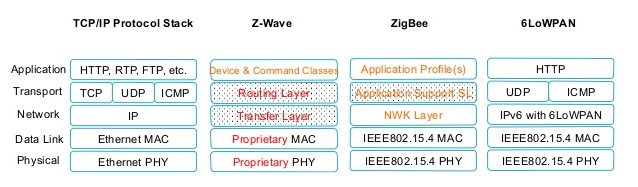
\includegraphics[width=15cm]{\rpDossier/images/comparison.jpg}
\caption{Comparaison de différents protocoles IoT}
\label{comparison}
\end{figure}

\todo[Mettre des observations pour zigbee et z-wave ?]

En réalité 6LoWPAN est plus une couche 2,5 que 3 ; en effet la couche 3 est IPv6. En fait, dans le cas de 6LoWPAN la pile réseau ressemble plus à celle présentée dans la \cref{stack6lowpan}.

\begin{figure}[H]
\centering
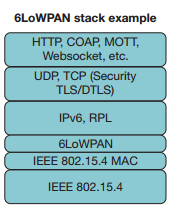
\includegraphics[width=5cm]{\rpDossier/images/stack6lowpan.PNG}
\caption{Stack 6LoWPAN}
\label{stack6lowpan}
\end{figure}

Comme nous pouvons voir, 6LoWPAN fait la liaison entre 802.15.4 et IPv6. Au niveau transport, 6LoWPAN supporte UDP et TCP, mais ce dernier n'est pas beaucoup utilisé. En effet, TCP étant un protocole connecté, les entête sont très grands (à cause de l'ajout de numéro de séquence par exemple) et donc pas vraiment pratiques pour les appareils basse consommation. Le trafic supplémentaire, avec les \textit{ACK}, rend son utilisation délicate. On privilégiera plutôt UDP et sa propre version de TLS, DTLS. 

Au niveau applicatif, il est bon de noter que 6LoWPAN supporte HTTP, mais ne l'utilise que très peu à cause de la verbosité du langage. L'industrie a développé un protocole de messagerie plus adapté au nom de \textbf{COAP} (\textit{COnstrained Application Protocol}) qui est beaucoup plus adapté aux appareils basse consommation.

% Compression des en-tête %
Du fait de la nécessiter d'optimiser la bande passante, et les données que l'on envoie, la compression des en-têtes est un enjeu essentiel de 6LoWPAN. De manière traditionnelle, la compression se fait quand plusieurs conditions sont réunies, si le flux de données entre deux équipements est stable.

La compression des en-tête est très efficace dans le cas d’un réseau statique mais perd son efficacité sur des réseaux dynamiques où l'en-tête doit être décompressée à chaque saut.

Quant on sait qu'un en-tête IPv6 classique fait quarante octets et que la longueur maximale d'une trame 802.15.4 est de cent-vingt-sept octets, il est plus que nécessaire de réduire la taille des en-têtes.

Dans le cas de 6LoWPAN, on peut atteindre 3 seuils de compressions :
\begin{itemize}
	\item 95~\% (2 octets) ;
	\item 70~\% (12 octets ;
	\item 50~\% (20 octets).
\end{itemize}

Pour être dans le cas optimal (compression de 95~\%), il faut que la communication se fasse entre deux appareils dans le même réseaux 6LoWPAN (point à point), qui utilise des adresses de lien local.

Pour obtenir une compression de 70~\%, il faut connaître l'identifiant réseau (de couche 2) de l'appareil dans le réseau et dans le pire cas (50~\%) on ne connaît que son adresse IPv6.

Dans le cas de 6LoWPAN, il existe deux types de routage (\cref{routing}), celui de niveau 3 et celui de niveau 2. Le premier utilise l'adresse IPv6 et le second l'adresse de niveau 2 (l'identifiant 802.15.4).

\begin{figure}[H]
\centering
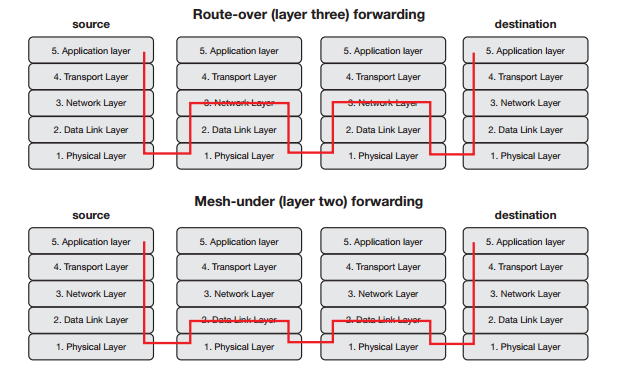
\includegraphics[width=15cm]{\rpDossier/images/routing.PNG}
\caption{Les deux types de routage avec 6LoWPAN}
\label{routing}
\end{figure}

Pour le  \textit{mesh-under} (couche 2), le routage des données est transparent, donc on peut considérer le réseau comme un sous-réseau IP. Le seul routeur IP dans cette configuration est l'\textit{edge router}. Un domaine de \textit{broadcast} est quand même défini pour garder la compatibilité avec le protocole IPv6 et conserver la détection de duplication d'adresse (DAD, \textit{Duplication Address Detection}), car ce type de message est diffusé sur tout le réseau et donc génère beaucoup de trafic. On privilégiera ce type de routage pour les réseaux de petite taille.

D'un autre côté, le routage de niveau 3 (\textit{route-over}) fait en sorte que chaque saut représente un routeur IP. Son utilisation est favorable dans le cas d’un grand réseau et dans l'optique de l'agrandissement de ce dernier. 

Dans le cas de 6LoWPAN, le protocole de routage de niveau 3 le plus utilisé est RPL (se prononce comme « \textit{ripple} »). En comparaison de \textit{mesh-under}, ce type de routage permet d'utiliser les protocoles qui ont pour standard la pile TCP/IP.

\textit{Routing Protocol for Low-power and Lossy network} (RPL) procure un mécanisme pour optimiser le \textit{multipoint-to-point} (différents capteurs qui veulent joindre le même serveur) et de la même manière le \textit{point-to-multipoint} (\textit{broadcast/multicast}).

\noindent RPL supporte deux modes de routages : 
\begin{itemize}
	\item \textit{storing mode}; 
	\item \textit{non-storing mode}.
\end{itemize}

En \textit{storing mode}, tous les appareils qui agissent comme routeur conservent une table de routage et une table de voisinage. La table de routage est utilisée pour sauvegarder les routes vers les différents appareils du réseau et la table de voisinage sert à garder une trace des voisins de l'équipement. 

Pour l'autre mode de fonctionnement, seul le \textit{border router} conserve une table de routage, ce qui permet d'utiliser du \textit{source routing}. Cela signifie que le paquet doit inclure la route complète pour atteindre sa destination. Par exemple, quand un appareil veut envoyer un paquet à un autre appareil du réseau 6LoWPAN, il envoie les données au \textit{border router}, qui regarde dans sa table de routage, ajoute la route au paquet puis envoie le paquet sur le réseau.

le \textit{storing mode} impose d'avoir des équipements plus robustes alors que l'autre augmente le nombre de sauts pour la transmission du paquet, ce qui peut potentiellement surcharger le réseau.

L'un des avantages d'IPv6 est l'auto-gestion des adresses : un appareil peut générer automatiquement son adresse sans avoir recours à un serveur DHCP. Le protocole \textbf{NDP} (\textit{Neighbor Discovery Protocol}) permet d'obtenir une adresse unique dans le réseau en évitant les conflits.

La sécurité dans l'IoT est un véritable défi ; en effet, à cause du nombre de nœuds avec des performances assez faible, il y beaucoup de points d'entrée pour les attaques de l'extérieur. Aussi l'un des points critiques dans l'IoT est la nature des données, qui dans certains cas peuvent être cruciales si elles servent à commander des alarmes ou des portes d'accès.

Du coup, 6LoWPAN tire parti de l'\textbf{AES-128} qui est définie dans 802.15.4. Avec l'utilisation de TLS ou de DTLS on peut aussi sécuriser les échanges au niveau de la couche transport, mais cela implique d'avoir des équipements avec une certaine puissance. Les cartes TI \textbf{CC 2538} fournis par notre tuteur ont été développées spécialement dans cette optique de sécurité.
